% system_overview.tex
% Compiled standalone with:  pdflatex -shell-escape system_overview.tex
% or with tectonic. Produces system_overview.pdf — convert to PNG via:
%   sips -s format png system_overview.pdf --out system_overview.png
\documentclass[tikz,border=10pt]{standalone}
\usepackage{amsmath,amssymb}
\usepackage{tikz}
\usetikzlibrary{positioning,arrows.meta,shapes.geometric,calc,fit,backgrounds,decorations.pathreplacing}

\begin{document}
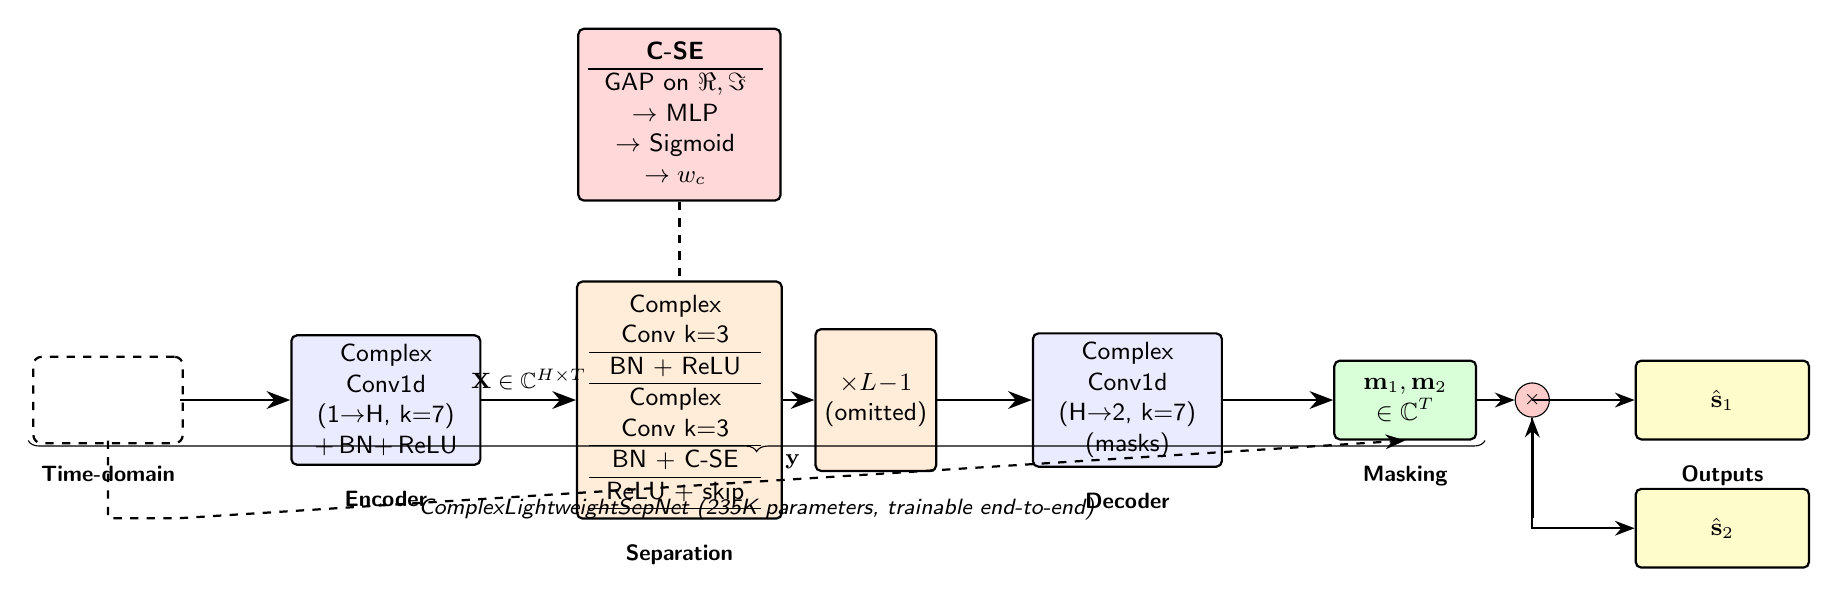
\begin{tikzpicture}[
    font=\sffamily\small,
    box/.style={draw, rounded corners=2pt, minimum height=10mm, minimum width=18mm, align=center, fill=blue!8, thick},
    resbox/.style={draw, rounded corners=2pt, minimum height=8mm, minimum width=14mm, align=center, fill=orange!15, thick},
    sebox/.style={draw, rounded corners=2pt, minimum height=6mm, minimum width=14mm, align=center, fill=red!15, thick},
    arrow/.style={-{Stealth[length=2.5mm]}, thick},
    bigarrow/.style={-{Stealth[length=3mm]}, line width=1pt},
    label/.style={font=\sffamily\footnotesize\itshape, fill=white, inner sep=1pt},
    stage/.style={draw, dashed, rounded corners=3pt, inner sep=4pt, thick}
]

% ===== Mixture =====
\node[box, fill=gray!15] (mix) at (0,0) {Mixture\\$\mathbf{y}\in\mathbb{C}^{T}$};

% ===== Encoder stage =====
\node[stage, fit=(mix), label=above:{Input}] (inputstage) {};

% ===== Encoder block =====
\node[box, right=14mm of mix, minimum width=24mm] (enc) {Complex\\Conv1d\\(1$\to$H, k=7)\\+\,BN+\,ReLU};

% ===== Residual block 1 =====
\node[resbox, right=12mm of enc, minimum height=18mm, minimum width=26mm, align=center] (res1) {
    \begin{tabular}{c}
    Complex \\ Conv k=3 \\ \hline
    BN + ReLU \\ \hline
    Complex \\ Conv k=3 \\ \hline
    BN + C-SE \\ \hline
    ReLU + skip \\ \hline
    \end{tabular}
};

% ===== Residual blocks 2,3,4 (compact) =====
\node[resbox, right=4mm of res1, minimum height=18mm, minimum width=14mm, align=center] (resdots1) {$\times L\!-\!1$\\ (omitted)};

% ===== Decoder block =====
\node[box, right=12mm of resdots1, minimum width=24mm] (dec) {Complex\\Conv1d\\(H$\to$2, k=7)\\(masks)};

% ===== Mask & multiply =====
\node[box, fill=green!15, right=14mm of dec, minimum width=18mm] (mask) {$\mathbf{m}_1,\mathbf{m}_2$\\ $\in\mathbb{C}^{T}$};

% ===== Outputs =====
\node[box, fill=yellow!20, right=20mm of mask, minimum width=22mm] (s1) {$\hat{\mathbf{s}}_1$};
\node[box, fill=yellow!20, below=6mm of s1, minimum width=22mm] (s2) {$\hat{\mathbf{s}}_2$};

% ===== C-SE detail box (above residual) =====
\node[sebox, above=10mm of res1] (cse) {
    \begin{tabular}{c}
    \textbf{C-SE} \\ \hline
    GAP on $\Re,\Im$ \\ $\to$ MLP \\ $\to$ Sigmoid \\ $\to w_c$ \\
    \end{tabular}
};
\draw[dashed, thick] (cse) -- (res1);

% ===== Arrows =====
\draw[bigarrow] (mix) -- (enc);
\draw[bigarrow] (enc) -- node[above, font=\footnotesize]{$\mathbf{X}\in\mathbb{C}^{H\times T}$} (res1);
\draw[bigarrow] (res1) -- (resdots1);
\draw[bigarrow] (resdots1) -- (dec);
\draw[bigarrow] (dec) -- (mask);

% branch: mixture copied to multiply
\coordinate (mixcopy) at ($(mix.east)+(0,-15mm)$);
\draw[arrow, dashed] (mix.south) |- (mixcopy) -- node[above, font=\footnotesize]{$\mathbf{y}$} (mask.south);

% multiply node
\node[draw, circle, fill=red!20, inner sep=1.5pt, font=\scriptsize] at ($(mask.east)+(7mm,0)$) (mul) {$\times$};
\draw[arrow, line width=1pt] (mask) -- (mul);
\draw[arrow, line width=1pt] (mixcopy -| mul) -- (mul);

% To outputs
\draw[arrow] (mul) |- (s1.west);
\draw[arrow] (mul) |- (s2.west);

% ===== Stage labels =====
\node[font=\sffamily\bfseries\footnotesize, below=2mm of mix] {Time-domain};
\node[font=\sffamily\bfseries\footnotesize, below=2mm of enc] {Encoder};
\node[font=\sffamily\bfseries\footnotesize, below=2mm of res1] {Separation};
\node[font=\sffamily\bfseries\footnotesize, below=2mm of dec] {Decoder};
\node[font=\sffamily\bfseries\footnotesize, below=2mm of mask] {Masking};
\node[font=\sffamily\bfseries\footnotesize, below=2mm of s1] {Outputs};

% ===== Stage brackets =====
\draw[decorate, decoration={brace, amplitude=4pt, mirror}] ($(mix.south west)+(-1mm,0)$) -- ($(mask.south east)+(1mm,0)$) node[midway, below=6mm, font=\sffamily\itshape\footnotesize, align=center]{ComplexLightweightSepNet (235K parameters, trainable end-to-end)};

\end{tikzpicture}
\end{document}